\begin{figure}[htbp]
  \centering
  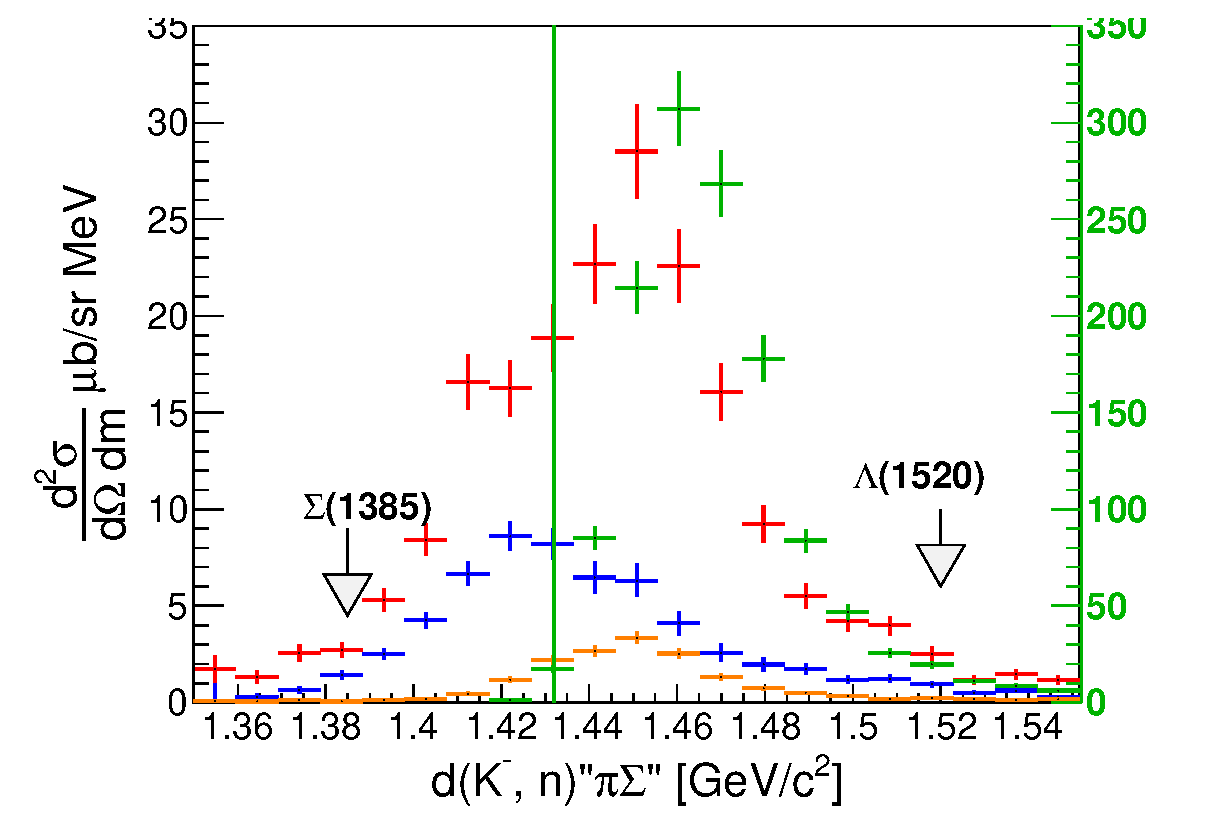
\includegraphics[width=8cm]{../pic/Dron/All_CS.eps}
  \caption{
    The obtained cross sections are plotted simultaneously in this figure.
    The $d(K^-, n)"\pi^-\Sigma^+$, $d(K^-, n)"\pi^+\Sigma^-"$, $d(K^-, n)"n K^0"$, and $d(K^-, p)"\pi^- \Sigma^0"$ plot as red, blue, green, and orange, lines respectively.
    The $d(K^-, n)"n K^0"$ is scaled to 1/10.
    The green virtical line indicates the $\bar{K}N$ threshold.
  }
  \label{fig:all_CS}
\end{figure}


The $d(K^-, n)\pi^{\mp}\Sigma^{\pm}$ and $d(K^-, p)\pi^-\Sigma^0$ spectra obtained through the procedures described in the previous section
are shown together in Figure \ref{fig:all_CS}.
In this figure, the green vertical line indicates the $\bar{K}N$ threshold.
This section discusses the qualitative features of the obtained spectra.

The experiment is interpreted as a two-step reaction, as described in Section \ref{sec:E31}.
The $\pi^-\Sigma^0$ spectrum contains only the $I=1$ component from the second-step scattering,
and this second-step scattering does not exhibit a significant structure, as there is no pole near the $\bar{K}N$ threshold.
As a result, the $\bar{K}N$ spectrum reflects the first-step scattering more directly.
A bump-like shape emerges from the $\bar{K}N$ threshold due to the Fermi motion of the spectator.

For the $I=0$ component, the second-step scattering is expected to exhibit a pronounced structure below the $\bar{K}N$ threshold
due to the presence of poles in that region.
This results in a spectral shape with a stronger enhancement below the $\bar{K}N$ threshold compared to the bump-like feature originating
from the first-step scattering.
Indeed, the observed $\pi^{\mp}\Sigma^{\pm}$ spectra, which contain both $I=0$ and $I=1$ components as well as their interference,
exhibit a clear structure below the $\bar{K}N$ threshold.
The overall spectral intensity is also larger than that of the $\pi^-\Sigma^0$ spectrum,
which only contains the $I=1$ component, due to the pole contribution in the $I=0$ channel.
The interference between the $I=0$ and $I=1$ components appears as a difference between the $\pi^-\Sigma^+$ and $\pi^+\Sigma^-$ spectra.
Since the measured spectra show a clear asymmetry between them,
the interference effect between $I=0$ and $I=1$ was observed in the reactions in this experiment.

In the second-step scattering near the $\bar{K}N$ threshold,
$S$-waves are expected to dominate due to the small angular momentum transfer transfer.
However, it is well known that in this region there are $I=0$ $D$-wave resonances, such as the $\Lambda(1520)$,
and $I=1$ $P$-wave resonances, such as the $\Sigma(1385)$.
The absence of structures around the $\Sigma(1385)$ region in the measured $I=1$ $\pi^-\Sigma^0$ spectrum,
as well as around both the $\Sigma(1385)$ and $\Lambda(1520)$ regions in the $\pi^+\Sigma^-$ and $\pi^-\Sigma^+$ spectra
with mixed $I=0$ and $I=1$ contributions, confirms that the $S$-wave dominates in the reactions observed in this experiment.

